\documentclass[10pt,a4paper]{article}

\usepackage[utf8]{inputenc}
\usepackage[T1]{fontenc}	
\usepackage[italian]{babel}
\usepackage{amsmath}
\usepackage{amsfonts}
\usepackage{amssymb}
\usepackage{graphicx}

\usepackage[left=2cm,right=2cm,top=2cm,bottom=2cm]{geometry}
\geometry{a4paper}

\usepackage{booktabs} % for much better looking tables
\usepackage{verbatim}
\usepackage{subfig} % make it possible to include more than one captioned figure/table in a single 

\usepackage{fancyhdr} % This should be set AFTER setting up the page geometry
\pagestyle{fancy} % options: empty , plain , fancy
\renewcommand{\headrulewidth}{0pt} % customise the layout...
\lhead{}\chead{}\rhead{}
\lfoot{}\cfoot{\thepage}\rfoot{}

%%% SECTION TITLE APPEARANCE
\usepackage{sectsty}
%\allsectionsfont{\sffamily\mdseries\upshape} % (See the fntguide.pdf for font help)
% (This matches ConTeXt defaults)

% pacchetti che mi fanno schifo ma uso lo stesso (Bob è scemo, ma anche Ale...)
\usepackage[cdot, thickqspace, squaren]{SIunits}
% il miglior pacchetto che potessi desiderare
\usepackage{float}
% macro che mi piacciono
\def\code#1{\texttt{#1}}


\title{Esperienza di Franck Hertz}
\author{Gruppo BL \\ Candido Alessandro, Luzio Andrea, Mazziotti Fabrizio}

\begin{document}

\maketitle

\begin{abstract}
Lo scopo di questa esperienza è di verificare la struttura discreta dei livelli energetici degll'atomo di neon e di stimare la sua energia di eccitazione.
\end{abstract}

\section{Strumentazione }

\begin{itemize}
 \item Oscilloscopio digitale Tektronix TDS 1012.
 		%Lo strumento è affetto da errore sistematico del 3 \% sulle scale di tensione utilizzate, e di 100 ppm sulle scale di tempo utilizzate.
 \item Tetrodo a gas neon ELWE U8482230
 \item Sistema di alimentazione e lettura di corrente ELWE

\end{itemize}

\section{Osservazione degli effetti degli urti anelastici elettrone-neon}

Dopo aver eseguito la procedura di accensione suggerita per l'apparato schematizzato in \figurename{~\ref{fig:circuito}},si è osservata la struttura luminosa nel tetrodo a gas al variare delle tensioni $U_{A}$ e $U_{G}$.

\begin{figure}[h!]
	\centering
		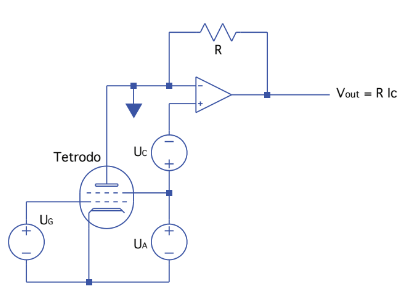
\includegraphics[width=0.80\textwidth]{../grafici/schema_apparato.png}
	\caption{Schema dell'apparato utilizzato nell'esperienza.}
	\label{fig:circuito}
\end{figure}

Come ci si aspetta, mantenendo fisso $U_{G}$ e aumentando la tensione anodica si osserva la comparsa di bande luminose nella parte arancione dello spettro.
Viceversa fissata la tensione anodica e diminuendo $U_{G}$ si ottengono gli stessi risultati, infatti ciò che conta per accelerare gli elettroni e permettergli di fare urti anelastici con il neon (cioè per far si che l'energia degli elettroni sia superiore alla differenza di energia tra due livelli energetici) è la differenza di potenziale $(U_{A}-U_{G})$.
La presenza della griglia di controllo permette di definire una superficie equipotenziale, così è come se gli elettroni venissero accelerati all'interno di un condensatore a facce piane parallele. Si può notare che diminuendo la tensione ai capi di questa griglia fino a 0, ad un certo punto le bande risultano distorte, in particolare diventando più spesse al centro del tetrodo. Questo è dovuto al fatto che in assenza di potenziale sulla griglia di controllo, il campo elettrico non è proprio uniforme in tutta la regione, tranne al più nella zona centrale, e quindi la maggior parte degli elettroni che non urtano con le pareti laterali del tetrodo saranno proprio quelli accelerati nella zona centrale.

% i potenziali U_G ecc li mettiamo senza errore o il manuale dice qualcosa in merito?

Si è fissato $U_{G} = \unit{3.8 \pm ???}{V}$, $U_{F}=\unit{8.0 \pm ???}{V}$, $U_{E} = \unit{10.6 \pm ???}{V}$(la tensione frenante è irrilevante perchè la misura è stata effettuata con il sistema di alimentazione e non con l'oscilloscopio) e si sono cercate le tensioni $U_{A}$ per le quali compare nelle immediate vicinanze della griglia anodica la prima banda luminosa, la seconda, etc. La comparsa delle bande corrisponde ai valori massimi della corrente $I_{C}$. Poichè le misure sono state effettuate ad occhio nudo, si sono stimati gli errori su di esse valutando la tensione minima e massima per cui si vedeva la comparsa di una banda. I risultati sono riportati in \tablename{~\ref{tab:massimi}}.

\begin{table}[h!]
\centering
\begin{tabular}{c|c|c|c|c}
\hline
Banda &1&2&3&4\\
\hline 
$U_{A} (V)$ & 22.5$\pm$1.5 & 41.0$\pm$1.5 & 54.5 $\pm$1.0 & 72.0$\pm$4.0  \\ 
\hline
\end{tabular}
\captionof{table}{Tensioni $U_{A}$ a fissato $U_{G}$ per cui si osservano le varie bande luminose nelle immediate vicinanze della griglia anodica.}
\label{tab:massimi}
\end{table}


%In prima approssimazione ci si aspetta che 
%\begin{equation}
%\frac{(U^{i+1}_{A}-U^{i}_{A})}{i} - U_{G} \approx E_{1}
% \end{equation}
%(i=1,2,3) cioè la differenza di potenziale tra le due griglie è circa uguale all'energia del primo livello energetico del neon.

%non so se scrivere questa cosa dato che non è vera, rappresenta solo una stima grezza, si dovrebbe confrontare con i risultati dell'analisi dei dati e poi motivare la discrepanza.

In secondo luogo si è attivato il generatore di rampa per $U_{A}$ e si è posto l'oscilloscopio in modalità normale  per osservare la curva $I_{C}$ vs $U_{A}$ (la stessa curva si può osservare in modalità X-Y, dove X = $U_{G}$/10 e Y $\propto I_{C}$) e la rampa, facendo attenzione a regolare il guadagno dell'opamp in modo da non saturarne l'uscita. L'andamento è mostrato in figura~\ref{andamento}.

\begin{figure}[h!]
	\centering
		\includegraphics[width=0.80\textwidth]{../oscilloscopio/correnteanodicatempo1.png}
	\caption{Curva $I_{C} - U_{A}$ con rampa per il potenziale $U_{A}$. I valori dei potenziali sono: $U_{F}=\unit{8}{V}$, $U_{E}=\unit{9.6}{V}$, $U_{G}=\unit{3.9}{V}$.}
	\label{andamento}
\end{figure}


All'aumentare di $U_{A}$, la corrente $I_{C}$ cresce fino a raggiungere un massimo quando l'energia degli elettroni è in grado di eccitare gli atomi di neon(comparsa della prima banda). La presenza del campo frenante dovuto al potenziale $U_{E}$ non permette a questi elettroni, che hanno perso energia in seguito all'urto, di arrivare all'anodo e quindi la corrente registrata diminuisce. la corrente $I_{C}$ ha un minimo quando la banda luminosa si distacca dalla griglia anodica, segno del fatto che gli elettroni hanno perso troppa energia per eccitare di nuovo il neon.
Aumentando ancora $U_{A}$ la corrente reinizia ad aumentare fino a raggiungere un nuovo massimo(comparsa della seconda banda) e così via.
Agendo sulla manopola del potenziale $U_{E}$ si è osservato il variare della curva $I_{C}$ vs $U_{A}$ al variare di $U_{E}$ ottenendo come risultati curve simili alla figura~\ref{andamento}, come ad esempio quella mostrata in figura~\ref{task5}.


\begin{figure}[h!]
	\centering
		\includegraphics[width=0.80\textwidth]{../oscilloscopio/task5.png}
	\caption{Curva $I_{C} - U_{A}$ per $U_{E}=\unit{11.9}{V}$.}
	\label{task5}
\end{figure}



All'aumentare di $U_{E}$ anche parte degli elettroni che fanno urti elastici con gli atomi di neon non giungono sull'anodo..%da finire
  
%ok, ma perchè abbiamo correnti negative? inoltre mi sembra che la discesa dopo il terzo massimo sia molto più lunga e la risalita molto più breve di quelle con Ue più piccolo.
%\\FINE PUNTO 5

 \subsection{}


\end{document}